\documentclass[12pt]{report}

\usepackage[T1]{fontenc}
\usepackage[utf8]{inputenc}
\usepackage{graphicx}
\usepackage{amsmath,amssymb,amsfonts}
\usepackage{txfonts}
\usepackage{pdfpages}
\usepackage{hyperref}

\renewcommand{\chaptername}{Rozdział}
\renewcommand{\contentsname}{Spis treści}
\renewcommand{\figurename}{Rys.}
\renewcommand{\tablename}{Tab.}
\renewcommand{\listfigurename}{Spis rysunków}
\renewcommand{\listtablename}{Spis tabel}
\renewcommand{\bibname}{Bibliografia}

\pagestyle{headings}

\setlength{\textwidth}{14cm}
\setlength{\textheight}{20cm}

\newtheorem{definition}{Definicja}
\newtheorem{example}{Przykład}[chapter]
\newtheorem{corollary}{Wniosek}[chapter]

\begin{document}

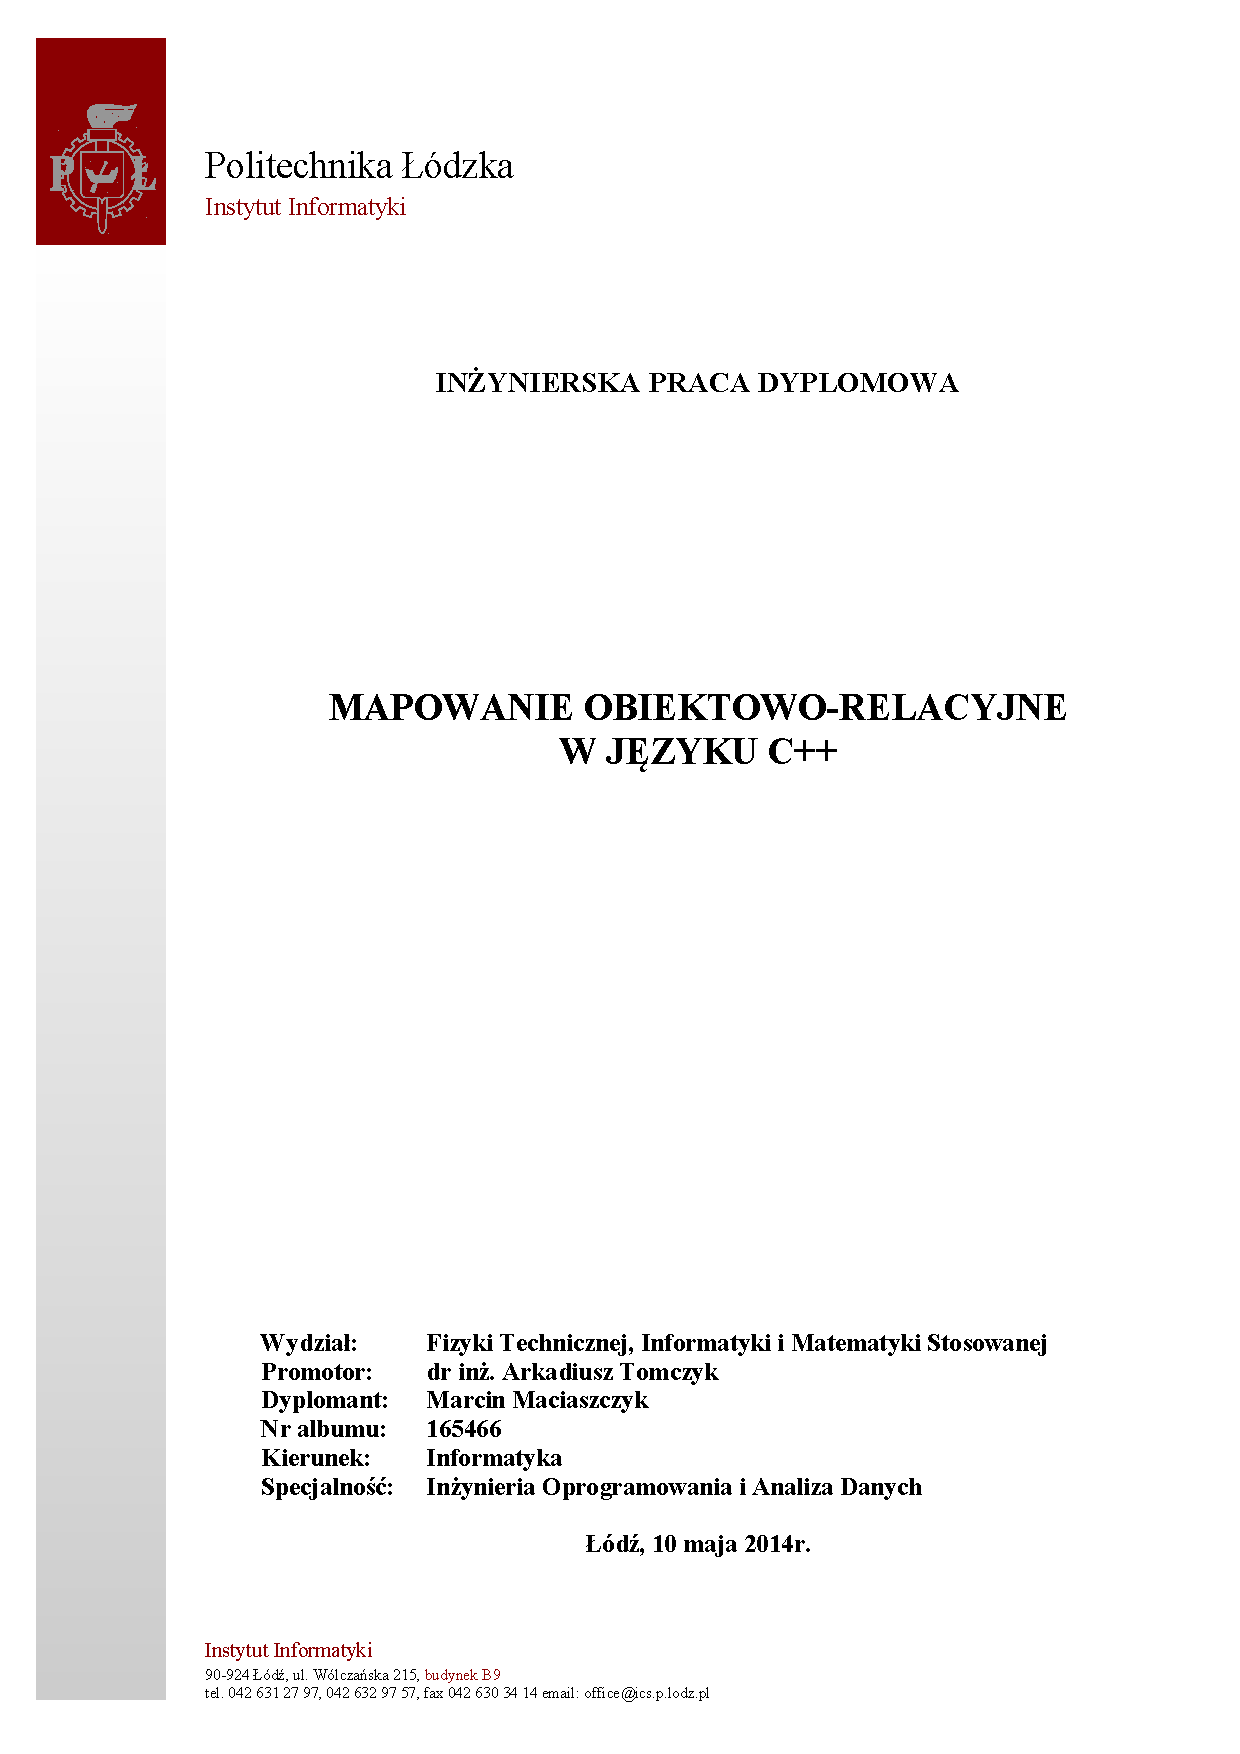
\includepdf[pages={1}]{resources/title_page.pdf}

\tableofcontents

\chapter{Wstęp} \label{wstep}

\section{Uzasadnienie wyboru tematu}

Wraz z rozwojem informatyki proces tworzenia oprogramowania wymaga od informatyków co raz większej wiedzy w poszczególnych dziedzinach takich jak na przykład bazy 
danych czy sieci komputerowe. Ciężko jest być specjalistą w każdej z nich, dlatego też podczas tworzenia oprogramowania programiści co raz częściej sięgają po różnego 
rodzaju narzędzia programistyczne, które mają za zadanie ułatwić im pracę. 

Przykładem takich narzędzi są aplikacje szkieletowe wykorzystywane jako fundamenty dla tworzonych aplikacji czy też biblioteki programistyczne udostępniające zestawy 
określonych funkcji. Oczywiście nie zawsze mamy możliwość skorzystania z wspominanych narzędzi, jednak jeśli taka istnieje warto wziąć to pod uwagę podczas fazy planowania 
tworzenia  oprogramowania, ponieważ decydując się na korzystanie z nich jesteśmy w stanie zaoszczędzić sporo czasu, a także uniknąć wielu błędów związanych z nieznajomością 
danej dziedziny.

Wraz z kolegą z tego samego roku studiów -- Sebastianem Florkiem, zdecydowaliśmy się w ramach pisamia pracy dyplomowej na wspólne stworzenie aplikacji szkieletowej, 
która będzie realizowała mapowanie obiektowo-relacyjne w języku C++. Wybór C++ jako języka programowania tłumaczymy dość dobrą jego znajomością, a także pewnym
doświadczeniem w programowaniu w tym języku nabytym w trakcie studiów. Mapowanie obiektowo-relacyjne jest to obecnie zagadnienie bardzo powszechne, szczególnie w 
językach programowania takich jak C\# czy Java. Programiści C++ nie mają już tak dużego wyboru wśród dostępnych narzędzi służących do mapowania 
obiektowo-relacyjnego, co także braliśmy pod uwagę ustalając temat nad jakim będziemy pracować.

Podział naszej pracy zostanie opisany w dalszych rozdziałach, jednak na wstępie warto zaznaczyć, że tematem pracy Sebastiana jest generator opisu mapowania 
obiektowo-relacyjnego, który jest wstępnym etapem pracy naszej aplikacji szkieletowej. Celem wspomnianego generatora jest wygenerowanie pliku projektu, a także plików
nagłówkowych oraz klas na podstawie istniejącej już bazy danych. Moim zadaniem będzie samo mapowanie obiektowo-relacyjne, które będzie się opierało na wcześniej
wygenerowanych plikach. 

\section{Problematyka i zakres pracy}

Programowanie obiektowe jest obecnie jednym z najpopularniejszych pa\-ra\-dy\-gma\-tów programowania, a pojęcia takie jak klasa czy obiekt znane są wszystkim programistom.
Podobnie jest z relacyjnym modelem organizacji baz danych i terminami takimi jak relacja czy krotka. Chcąc wykorzystać oba te podejścia w jednej aplikacji musimy zadbać o 
obustronną konwersję pomiędzy danymi z tabel relacyjnej bazy danych a obiektami aplikacjii. Tym właśnie zajmuje się mapowanie obiektowo-relacyjne, które wraz z tworzeniem 
aplikacji szkieletowych w języku C++ jest główną problematyką niniejszej pracy.

W tym momencie powstaje pytanie czy na prawdę warto korzystać z bibliotek i aplikacji szkieletowych służących do mapowania obiektowo relacyjnego? Od\-po\-wiedź nie jest
jednoznaczna w wszystkich przypadkach, ale warto wymienić jego podstawowe wady i zalety, których dokładniejsza analiza znajduje się w dalszej części pracy. Zacznijmy od zalet 
wykorzystania narzędzi ORM\footnote{mapowanie obiektowo-relacyjne (ang. Object-Relational Mapping)}:

\begin{itemize}
\item Znacznie zredukowana ilość pracy wymagana na oprogramowanie dostępu do bazy danych.
\item Nieobowiązkowa znajomość języka SQL\footnote{strukturalny język zapytań (ang. Structured Query Language)}. W celu tworzenia zapytań do bazy
danych korzystamy z interfejsu udostępnianego przez daną bibliotekę czy też aplikację szkieletową.
\item Uniezależnienie się od rodzaju systemu zarządzania bazą danych, możemy korzystać równie dobrze z MySQL, Oracle, PostgreSQL czy też Microsoft SQL Server
niekoniecznie posiadając o nich rozbudowaną wiedzę.
\item Aby skorzystać z transakcji, połączenia z bazą danych a także wieu innych funkcjonalności baz danych wystarczy zazwyczaj wywołać pojedyńczą me\-to\-dę.
\item Cały model danych przechowywany jest w jednym miejscu oraz nie jest ściśle związany z wykorzystywanym systemem zarządzania bazą danych dzięki cze\-mu łatwiej 
jest nam wprowadzać kolejne modyfikacje w kodzie oraz nawet zmieniać system zarządzania bazą danych na inny.
\end{itemize}

Wszędzie gdzie pojawiają się zalety mamy też do czynienia z wadami, nie inaczej jest w tym przypadku:

\begin{itemize}
\item Konfiguracja jest najczęściej skomplikowana i wymaga sporo czasu.
\item Podobnie jest z użytkowaniem, aby robić to w sposób optymalny musimy dobrze poznać daną bibliotekę czy też aplikację szkieletową.
\item Proste zapytania są obsługiwane bardzo sprawnie, jednak gdy przetwarzamy duże ilości złożonych zapytań wydajność nie dorówna nigdy zapytaniom na\-pi\-sa\-nym
przez specjalistę znającego język SQL.
\item Abstrakcja wprowadzona przez narzędzia ORM może okazać się uciążliwa, ponieważ nie zawsze zdajemy sobie sprawę z tego co dzieje się za kulisami w trakcie
wykonywania poszczególnch operacji.
\end{itemize}

Naszym głównym celem jest uczynienie Qubica dobrą alternatywą dla nie\-li\-cznych, ale istniejących już bibliotek oraz aplikacji szkieletowych realizujących mapowanie 
obiektowo-relacyjne w języku C++. Wszystkie nam obecnie znane rozwiązania są dostępne za darmo, jednak nie udostępniają one generatora opisu będącego w stanie 
wygenerować cały projekt aplikacji a ich interfejsy nie należą do intuicyjnych. Wprowadzenie generatora oraz intuicyjnego interfejsu użytkownika powinno uczynić Qubica
istotną alternatywą dla istniejących już narzędzi.

Analizę istniejących rozwiązań przedstawia kolejny rozdział a zestawienie z rezultatami naszej pracy znajduje się natomiast w końcowej części pracy, gdzie zostaną
przedstawione uzyskane przez nas wyniki oraz podsumowanie wykonanej przez nas pracy.

\section{Cele pracy} % Podrozdział około 1 strony, czyli 1800 znaków. Każdy cel opisany w 2-3 zdaniach, bez używania skrótów.

Do najważniejszych celów niniejszej pracy dyplomowej należą:

\begin{itemize}
\item Analiza istniejących bibliotek oraz aplikacji szkieletowych realizujących ma\-po\-wa\-nie obiektowo-relacyjne w języku C++.
\item Stworzenie własnej aplikacji szkieletowej realizującej mapowanie obiektowo-relacyjne w języku C++.
\item Analiza porównawcza szybkości działania przykładowej aplikacji stworzonej w oparciu o Qubic a o inne istniejące narzędzia.
\item Analiza porównawcza ilości kodu przykładowej aplikacji stworzonej w oparciu o Qubic a o inne istniejące narzędzia.
\end{itemize}

Do celów części praktycznej należą:

\begin{itemize}
\item Stworzenie intuicyjnego interfejsu użytkownika -- aby sprawdzić w jakim stopniu udało się zrealizować założenia zostanie przeprowadzony test po\-le\-ga\-ją\-cy na napisaniu
tej samej aplikacji wykorzystującej Qubica oraz inne aplikacje szkieletowe i bibioteki, a następnie porównaniu ilości linii kodu stworzonych aplikacji.
\item Stworzenie generatora opisu mapowania obiektowo-relacyjnego -- jest to przed\-mio\-tem pracy Sebastiana, naszym wspólnym celem jest integracja obu modułów.
\item Poprawne zrealizowanie założeń mapowania obiektowo-relacyjnego, a także jak najlepsza optymalizacja zapytań -- aby sprawdzić w jakim stopniu udało się zrealizować
założenia zostanie przeprowadzony test polegający na napisaniu tej samej aplikacji wykorzystującej Qubica oraz inne aplikacje szkieletowe i bibioteki, a następnie porównaniu
ich wydajności.
\item Uczynienie konfiguracji Qubica jak najprostszą.
\end{itemize}

\section{Metoda badawcza}

\subsubsection{Studia literaturowe} % Podrozdział około 1 strony, czyli 1800 znaków.Opis w 2-3 zdaniach. Wymagane odniesienia do bibliografii!

Podstawowa literatura wykorzystana podczas pisania niniejszej pracy dotyczy specyfikacji języka C++ oraz zapytań w języku SQL, są to powszechne zagadnienia, więc wybór
pozycji książkowych jest spory. Materiały dotyczące samego mapowania obiektowo-relacyjnego czy też aplikacji szkieletowej Qt pochodzą głównie z źródeł elektronicznych w 
języku angielskim, co jest związane z mniejszą popularnością tych tematyk.

\subsubsection{Analiza istniejących rozwiązań}

Analiza istniejących rozwiązań jest o tyle dobrą metodą badawczą, że stosując ją poznajemy praktyczne rozwiązania konkretnych problemów, czyli coś czego nie daje nam w
żaden sposób teoria.

\subsubsection{Stworzenie własnej aplikacji szkieletowej}

Praktyka jest najczęściej najlepszą z dostępnych metod nauki i to właśnie podczas tworzenia własnej aplikacji szkieletowej realizującej mapowanie obiektowo-relacyjne można
się najbardziej z danym tematem zapoznać. Wszystkie problemy, które pojawiały się poczas pisania Qubica musiały zostać w pewien sposób roz\-wią\-zane i to właśnie analiza
tych problemów i ich rozwiązywanie było główną metodą badawczą wykorzystaną podczas pisania niniejszej pracy.

\subsubsection{Analiza porównawcza oraz testy}

Analizując wcześniej istniejące już rozwiązania i powównując je z własnym można dojść do najtrafniejszych wniosków. To właśnie na tym etapie często dowiadujemy się czy
przyjęte przez nas założenia i zaproponowane rozwiązania były lepsze niż te z istniejących już rozwiązań. 

\section{Przegląd literatury w dziedzinie}

\subsubsection{Literatura dotycząca języka C++}

\subsubsection{Literatura dotycząca języka SQL}

\subsubsection{Literatura dotycząca mapowania obiektowo-relacyjnego}

\subsubsection{Literatura dotycząca aplikacji szkieletowej Qt}

\section{Układ pracy} % Cały podrozdział około 1 strony.

Tematem niniejszej pracy jest mapowanie obiektowo-relacyjne w języku C++, zaś za jej główny cel przyjęto przeanalizowanie istniejących bibliotek oraz aplikacji szkieletowych
realizujących mapowanie obiektowo-relacyjne oraz zaproponowanie własnej aplikacji szkieletowej.

W rozdziale \ref{wstep} uzasadniony został wybór tematu pracy, opisane jej cele oraz problematyka i zakres. Rozdział \ref{teoria} zawiera opis zagadnień teoretycznych
do\-ty\-czą\-cych mapowania obiektowo-relacyjnego a także tworzenia aplikacji szkieletowych w języku C++.

Najważniejszym rezultatem pracy jest analiza oraz porównanie istniejących bibliotek programistycznych i aplikacji szkieletowych realizujących mapowanie obiekt\-owo-rel\-acyjne
z stworzonym przez nas Qubiciem.

\chapter[Zagadnienia teoretyczne]{Zagadnienia teoretyczne dotyczące mapowania obiektowo-relacyjnego oraz aplikacji szkieletowych} \label{teoria}

\section{Podstawowe definicje} % Dokładny opis terminologii  pojęć zasadniczych dla tematu pracy, którymi autor będzie się posługiwał przy realizacji głównych celów pracy.

\chapter{Technologie i metody użyte w części badawczej} \label{technologie} % Sprzęt, oprogramowanie, serwer bazy danych, technologie i metodologie, język, biblioteki, wzorce.

\chapter[Analiza istniejących rozwiązań]{Analiza istniejących rozwiązań mapowania obiektowo-relacyjnego w języku C++} \label{analiza}

\chapter{Aplikacja szkieletowa Qubic} \label{qubic}

\section{Analiza wymagań} % Studium możliwości, wymagania funkcjonalne, niefunkcjonalne i ograniczenia projektu.

\section{Projekt} % Projekt wartswy danych, logiki i widoku. Diagramy klas, wzorce projektowe. Rodzaj aplikacji, wybór środowiska i platformy działania. Wybór bibliotek.

\section{Implementacja} % Punkty kluczowe, rodzaje przeprowadzanych testów.

\section{Konserwacja i inżynieria wtórna} %Jak przebiega eksploatacja projektu? Jakie wady i zalety ujawniły się po okresie testowania i użytkowania?
% Jak można skorzystać z tej wiedzy praktycznej pod kątem roz\-bu\-do\-wy pracy? Jakie elementy systemu powinny zostać w pierwszej kolejności zmodyfikowane?  

\section{Dokumentacja użytkownika}

\section{Przykładowa aplikacja wykorzystująca Qubica}

\section{Testy oraz ich wyniki}

\section{Perspektywy rozwoju Qubica}

W celu dalszego rozwoju stworzonej aplikacji szkieletowej warto rozważyć wprowadzenie następujących usprawnień:

\begin{itemize}
\item System adnotacji -- obecnie na opis mapowania składają się odpowienie nazwy funkcji oraz makra Qt. Istnieje jednak możliwość wprowadzenia własnych makr, które
miałyby opisywać mapowanie pomiędzy nazwami tabel z baz danych a odpowiednimi polami klas napisanych z języku C++. Dzięki temu zaistniałaby możliwość uniezależnienia
nazw pól klas od nazw tabel w bazie danych.
\item Interfejs zapytań -- choć jest już zaimplementowany, nadal nie udostępnia on wszystkich możliwych funkcjonalności języka SQL. Implementacja obsługi takich poleceń
jak JOIN czy UNION z pewnością byłaby dodatkowym atutem.
\item Identyfikacja tabel także za pomocą kluczy złożonych -- w tej chwili tabele identyfikowane są za pomocą kluczów głównych, co z kolei wymusza ich nadawanie w każdej
z tabel.
\item Pamięć podręczna -- wprowadzenie pamięci podręcznej może znacznie polepszyć wydajność w przypadku ciągłych operacji na tych samych danych.
\item Konfiguracja z poziomu kodu -- obecnie większość konfiguracji jest zapisana w plikach konfiguracyjnych i tylko tam może być zmieniana, w celu rozwoju wprowadzenie
dodatkowej możliwości jego konfiguracji wydaje się być dobrym pomysłem.
\item Wsparcie dla różnych rodzajów baz danych -- wprowadzenie tego usprawnienia ogranicza się do implementacji kilku interfejsów dla innych niż MySQL rodzajów baz 
danych. Biorąc pod uwagę możliwość wzorowania się na zaimplementowanej już logice nie powinno to stworzyć problemu gdy zaistnieje taka konieczność.
\item Serializacja danych -- dodanie możliwości serializacji może okazać się użyteczne w przypadku pracy z dużymi ilościami danych, w tym celu można skorzystać z wielu
istniejących już bibliotek udostępniających tę możliwość.
\item Internacjonalizacja -- w tej chwili wszystkie logi zlokalizowane są w języku angielskim, istnieje jednak możliwość zmiany obecnego stanu poprzez wykorzystanie modułu
translacji udostępnianego przez Qt.
\item Wielowątkowość -- wykorzystanie wielowątkowości w przypadku mapowania-obiektowo relacyjnego z pewnością nie należy do najłatwiejszych zadań, jednak znacznie
może to usprawnić wykonywanie bardziej wymagających operacji.
\end{itemize}

\chapter{Podsumowanie} \label{podsumowanie}

\section{Dyskusja wyników}

\section{Perspektywy rozwoju pracy} % Jak można kontynuować tę pracę, zwłaszcza pod kątem magisterskich i dalej? Co jeszcze powinno być zrobione lub ulepszone?
% Co należy zmienić lub poprawić w pracy z dzisiejszego punktu widzenia?

Dzięki zrealizowaniu pracy poprawie uległa wydajność. Ponadto, o ? \% skrócony został czas. Które cele pracy udało sie zrealizować? Co z tego wynika? Które cele pracy 
pozostały niezrealizowane i dlaczego? 

\addcontentsline{toc}{chapter}{Bibliografia} 
\begin{thebibliography}{99}
\bibitem{symfonia} Grębosz, Jerzy. Symfonia C++. Standard. Wyd. 3. Kraków, 2013. ISBN 978-83-7366-134-4.
\bibitem{cpp} C++ Language Tutorial. \url{http://www.cplusplus.com/doc/}.
\bibitem{sql} Viescas, John. SQL Queries for Mere Mortals. 2001. ISBN 83-7279-152-X.
\end{thebibliography}

\addcontentsline{toc}{chapter}{Spis rysunków} 
\listoffigures

\addcontentsline{toc}{chapter}{Spis tabel} 
\listoftables

\addcontentsline{toc}{chapter}{Załączniki} 
\chapter*{Załączniki}
\begin{enumerate}
\item
\end{enumerate}

\end{document}